\subsection{Chirp detection algorithm}

We developed and tested the improved algorithm on the raw data from a competition experiment (more information in section \ref{Behaviour}, or in the Paper by \cite{raabElectrocommunicationSignalsIndicate2021}) with 15 electrodes arranged in a grid. To be able to analyze the communication signals of the fish, which are most prominently represented as changes in their EOD$f$, we used the frequency tracks that were already computed by \textcite{raab2022AdvancesNoninvasiveTracking}. A frequency track is an approximation of how the fundamental frequency of the EOD of a single fish evolves. But because they are estimated using a spectrogram, they lack the temporal information needed to resolve transient frequency changes of a chirp. For this reason, we use the raw data, which has the appropriate temporal resolution to resolve chirps. To extract the EOD of single individuals, the frequency tracks are used to build specific band pass filters for every fish. Because the baseline EOD$f$ of a single fish changes with temperature and communication signals, filtering had to be performed in time windows. Additionally, to obtain the best signal for a freely moving fish, we choose the electrode with the highest power for every single rolling window. For each time window, we extract the amplitude of the baseline, the instantaneous frequency, and the amplitude of the search frequency, which all change during the production of a chirp. Simultaneously detected peaks on all three features are classified as a chirp. All signal processing steps that the raw data in a single rolling window snippet goes through are summarized in figure \ref{fig:algorithm}. The following paragraphs describe the processing steps in the same order as they are organized in the code of the algorithm. 

\subsubsection{Loading and preparing the data set}

The parameters used by the algorithm are all adjustable using a \codeword{yaml} configuration file, which includes sections for the path to the data set as well as to the output directory. The program loads the raw data as well as the frequency tracks for every fish in the recording and generates time windows, in which it iterates across the raw data set. For each window in time, it iterates through the respective windows on the frequency tracks of all the fish in the recording. This approach is arguably less intuitive compared to iterating through the full time of the recording on the frequency track of a single fish and then skipping to the next individual. However, it reduces the number of times the more memory- and hence computationally demanding raw data set needs to be loaded. 

\subsubsection{Rolling windows and their overlap}

To reduce the edge effects caused by filtering, we overlapped the rolling windows (window duration of \SI{5}{\second}) by one second and discarded the first and last \SI{250}{\milli\second} of a single window. This resulted in a true overlap of \SI{0,5}{\milli\second} in which chirps might be detected twice. To resolve this issue, we grouped all chirps that occurred less than \SI{20}{\milli\second} apart from each other as a single chirp. 

\subsubsection{Following a fish through space}

The raw data set was recorded using an electrode grid. Hence, the EOD amplitudes of single fish varies between electrodes, because the amplitude decreases with the distance between an electrode and a moving fish. These changes in amplitude convey information on where the individual of interest is located in space. For optimal detection of chirps, we should use the strongest electrode for one fish, since it should have the highest signal-to-noise ratio. Additionally, if multiple fish are further apart, it is advantageous to use the electrode that is closest to one fish, but not the other, to increase the odds of correct sender assignment. For each iteration of the algorithm, we start off with a short (\SI{5}{\second}) snippets of the approximated frequency track and respective powers of the frequencies of an individual fish on the same temporal extent. To decide upon which raw data snippet for this fish across the pool of 15 electrodes the algorithm should load for optimal performance, we first had to determine, to which electrode the fish was the closest in the current window in time. To determine the best electrodes, we simply use the ones that had the highest power in the tracked frequencies, since power is proportional to the amplitude squared. In the current implementation, we repeat the following pipeline for the two electrodes with the highest power for the current fish of interest. 

\subsubsection{Feature extraction}

After determining the best electrodes, we load the raw data snipped for the respective time window. This results in a data set of the frequency track of a fish (Figure \ref{fig:algorithm}, A, red)  and the raw data (Figure \ref{fig:algorithm}, A, spectrogram), which the algorithm uses to extract more information. For each frequency track of an individual fish in each window, the raw signal \SI{5}{\hertz} is then band pass filtered with cut off frequencies above and below the baseline of the frequency track. This effectively provides an approximation of the recorded signal as if the current fish was the only one in the area. However fast frequency excursions, e.g. during chirps, are lost because they exceed the frequency limits of the cutoff frequencies. In other words, the peak of the chirp is filtered out by the band pass filter and that is why we see a trough in the amplitude. We use this to our advantage because the amplitude of the signal drops at theses points in time. To use the amplitudes of this signal, we extract the envelope using a low pass (cut off at \SI{25}{\hertz}) filter multiplied by the square-root of two (Figure \ref{fig:algorithm}, B, red). In addition to the amplitude trough, a chirp should also change the frequency of the signal, even if the actual peak gets lost due to filtering. To detect such transient frequency changes, we also compute the instantaneous frequency of the filtered baseline, which can be achieved by extracting the inverse of every single period using the zero crossings of the signal (Figure \ref{fig:algorithm}, B, orange).  But using just the envelope and the instantaneous frequency of the EOD baseline of the fish was not sufficient to determine whether the anomaly we detected is a chirp or is caused e.g. by the movement of the fish. To deal with this issue, we used the notion that chirps are always up-modulations of the frequency that reach values of +\SI{50}{\hertz} to +\SI{300}{\hertz} above the baseline EOD$f$ of the emitting fish \parencite{zakonEODModulationsBrown2002a}. The first approach by \textcite{henningerStatisticsNaturalCommunication2018} was to filter a band at approximately +\SI{10}{\hertz} above the baseline and look for peaks in the power of this filtered band. We call this area the 'search frequency'. However, this method comes with the limitation, that if there are multiple fish and one of them has a baseline EOD$f$ that is coincidentally higher than the frequency of the current analyzed fish, the search frequency will become unusable. If the search frequency is close to- or at the baseline frequency of a fish with higher EOD$f$, chirps from the fish with a lower EOD$f$ would not be correctly assigned to the sender (Figure \ref{fig:henninger}). We adopted the method first documented in \textcite{henningerStatisticsNaturalCommunication2018} but introduce a dynamically adjusted search frequency. In our version of the chirp detection algorithm, the search frequency is still confined to a region of +\SI{20}{\hertz} to +\SI{100}{\hertz} above the baseline. In contrast to \textcite{henningerStatisticsNaturalCommunication2018} in this window, the frequency tracks of all other individuals are evaluated to find a region with the largest frequency difference from all other individuals that is still within the usual frequency peaks of chirps. The search frequency is then extracted in this window. This should make chirp detection and, most importantly, correct assignment to the sender, possible with recordings that include multiple individuals (Figure \ref{fig:dynamic}). The search window chosen in the example in Figure \ref{fig:algorithm}, A is indicated by orange dashed lines on the spectrogram. The envelope of the search frequency is visualized by the orange line in panel B. 

\begin{figure}[H]
    \centering
    
\includegraphics[width=\linewidth]{figures/henninger.pdf}
    \mycaption{Fixed search frequency}{Schematic sketch of a fixed search frequency used by \textcite{henningerStatisticsNaturalCommunication2018}. The search frequency is placed at a static \SI{10}{\hertz} above the baseline of the lower fish. \textbf{A:} If there is no upper fish with a higher EOD$f$ in the search frequency, a chirp detection can be implemented. The decrease in amplitude and the increase of amplitude in the search frequency can be used for the chirp detection algorithm. \textbf{B:}
    In the case that there is another fish with an EOD$f$ in the search frequency, chirp detection is impaired. The EOD at the search frequency contains the chirp of the lower fish and the EOD of the upper fish, which is making the detection of the chirp unreliable.}
    \label{fig:henninger}
\end{figure}

\begin{figure}[H]
    \centering
    \includegraphics[width=\linewidth]{figures/dynamic.pdf}
    \mycaption{Dynamic search frequency}{Schematic sketch of a dynamic search frequency implemented in the new algorithm. The search frequency is dynamic in a range of \SIrange{20}{100}{\hertz} above the baseline of the lower fish. \textbf{A:} If there is no upper fish with a higher EOD$f$ in the search frequency, chirp detection can be implemented. The decrease in amplitude and the increase of amplitude in the search frequency can be used for the chirp detection algorithm. \textbf{B:}
    In the case that there is another fish with an EOD$f$ in the search frequency, the search frequency changes dynamically to a space with the largest difference to the upper fish. The chirp assignment is now possible with a correct sender assignment.}
    \label{fig:dynamic}
\end{figure}

\subsubsection{Feature processing}

The features we extracted, particularly the filtered baseline EOD, are also subject to change e.g. when the fish moves. But changes due to movements happen on a larger time scale. To reduce the impact of this noise, we additionally band-pass filtered the baseline envelope with cutoff frequencies \SI{2}{\hertz} (low-cutoff) and \SI{100}{\hertz} (high-cutoff). Additionally, we invert the baseline envelope to turn troughs into peaks for detection purposes. For the instantaneous frequency, we took the absolute and shifted it by the median of the EOD$f$ ($|EODf_{inst} - med({EODf_{inst}}|$). The instantaneous frequency during a chirp was negative in some cases. This irregularity is discussed in section \ref{ref:insta}. 
The search frequency required no additional processing. The processed features are visualized in the panel C of Figure \ref{fig:algorithm}. We then detected the peaks of all three features using a prominence threshold of 0.00005 for the baseline envelope, 0.000004 for the search frequency, and 2 for the instantaneous frequency.

\subsubsection{Peak classification}

Since all three features should coincide temporally with the peak in frequency during a chirp, the first criterion for a chirp was that peaks were detected on all three features simultaneously. More specifically, we chose \SI{20}{\milli\second} as a tolerance window where the peaks must co-occur. Additionally, since we repeated the algorithm on the two electrodes of the highest power for the current time window, we set a threshold of the number of electrodes on which the chirp must appear to be accepted as a chirp. In the current implementation, the chirp must be detected on just a single electrode. If a chirp is detected we compute the mean of the three time points on which the peaks were found and appended the resulting time stamp to the chirp times of the current fish.

\begin{figure}[H]
    \centering
    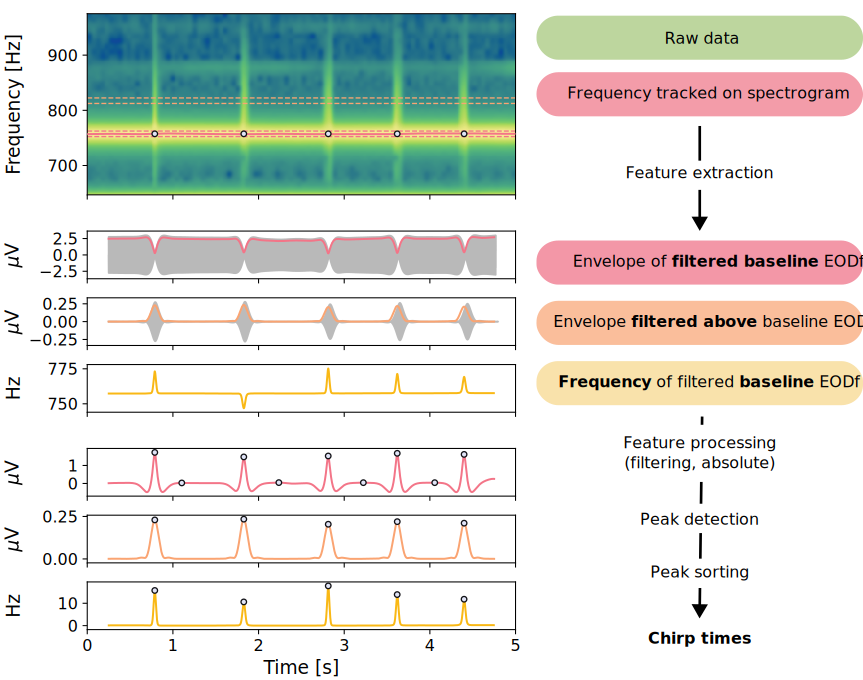
\includegraphics[width=\linewidth]{figures/10.0_11245.5.pdf}
    \mycaption{Core processing pipeline of the chirp detector.}{The left side shows how the data is modified while it passes the algorithm. The right side is color-coded with respect to the plots and indicates what kind of data is visualized and how it is processed. \textbf{A:} The spectrogram on the top is used to visualize the raw data. The red line on the spectrogram indicates the tracked frequency. \textbf{B:} The subplots show the three features that the algorithm extracts from the raw data using the frequency tracks of the individual fish. Red indicates the envelope of the baseline EOD$f$ for a single fish, which we obtain by filtering the raw signal around the tracked frequency. The envelope of the 'search frequency' we obtain by filtering a narrow band inside a dynamically adjusted window above the baseline EOD$f$ of the respective fish is indicated in orange. The search frequency band is also indicated by dashed lines in the same color on the spectrogram. The yellow line is the instantaneous frequency of the filtered baseline (red), which changes if the signal disappears out of the filtering window during a chirp. \textbf{C} illustrates how the three features appear after they are processed. The dots indicate the detected peaks. The dots on the spectrogram indicate the detected chirps after the peaks are sorted.}
    \label{fig:algorithm}
\end{figure}

\subsection{Behavioral data used to test the algorithm } \label{Behaviour}

We tested the algorithm on a data set published by \textcite{raabElectrocommunicationSignalsIndicate2021}. The dataset was recorded using 21 mature \textit{Apteronotus leptorhynchus} from a tropical fish supplier. 9 males and 12 females, all in non-breeding conditions, were used. The experiment was conceptualized to understand the role of rises, another communication signal, during the competition of two fish for a superior shelter. The experiments took place in a \SI{100}{\liter} tank with a superior shelter in the center surrounded by other, less optimal shelters. The bottom of the tank was equipped with 15 mono-polar electrodes with low-noise buffer headstages. A reference electrode was positioned in a corner of the tank. The electric signals were first amplified and then digitized at \SI{20}{\kilo\hertz} per channel. The movement of the fish was recorded by a video camera mounted above the aquarium. Behavior (chasing events and contacts) were annotated manually using the software package BORIS \parencite{https://doi.org/10.1111/2041-210X.12584}.

\subsection{Data analysis}

The chirp detection algorithm as well as our subsequent analysis were written in Python 3.10.9 using the packages numpy, scipy, matplotlib, \href{https://github.com/janscience/thunderfish}{thunderfish} and \href{https://github.com/janscience/audioio}{audioio} \parencite{2020SciPy-NMeth, Hunter:2007, harris2020array}. All scripts as well as the required package versions are publically available in a \href{https://whale.am28.uni-tuebingen.de/git/raab/GP2023_chirp_detection}{git repository} (\url{https://whale.am28.uni-tuebingen.de/git/raab/GP2023_chirp_detection}). The temporal relation between chirps and chasing events was analyzed using a cross-correlation analysis. We computed the temporal differences between agonistic events (chasing onset, -offset and contact) and the chirps up to $\pm$ \SI{90}{\second} before and after the event. We then convolved the temporal differences with a Gaussian kernel with a standard deviation of \SI{2}{\milli\second}. To generate a baseline to compare the convolution with we randomly shuffled the chirp intervals in 50 permutations and recomputed the convolution for each. The baseline distribution was then obtained by the median across the permutations with the 5th and 95th percentile respectively.